\documentclass[13pt]{article}
\usepackage[utf8]{inputenc}
\usepackage{amsmath}
\usepackage{comment}
\usepackage{physics}
\usepackage{mathrsfs}
\usepackage{graphics}
\usepackage{graphicx}
\usepackage{placeins}
\usepackage{caption}
\usepackage{subcaption}
\usepackage{color}
\usepackage{biblatex}
\addbibresource{bibliography.bib}
\title{Various aspects of the Fano resonance in nano-optical systems}
\author{Shyamal Guchhait}
\date{}
\begin{document}
	
	\maketitle
	
	\begin{abstract}
		The magneto-optical effects in hybrid magneto-plasmonic systems have been importanted because of their potential for building non-reciprocal nanophotonic devices as well as fundamental physics, for application need the large magneto-optical effects. Here, we unravel different physical origins of the giant enhancement of Faraday rotation and ellipticity in a hybrid magneto-plasmonic system, namely, waveguided magneto-plasmonic crystal for excitation with transverse electric (TE) and transverse magnetic (TM) polarized light. With TE polarization excitation, quasi waveguide mode is dominated. Here, the natural weak value amplification is the dominant cause of the enhancement of Faraday effects appearing due to the spectral domain interference of Fano resonance. For TM polarization excitation, waveguide-plasmon strong coupling and its universal manifestation of avoided crossing play an important role, leading to the Faraday effects enhancement near the avoided crossing regime.
		\par
		The valley degree of freedom possessed by electronic excitations in transition metal dichalcogenides is providing new opportunities for information processing and optoelectronics. Valley contrasting polarization selection rules present unique opportunities for optical control in valleytronic devices. Critical to devices leveraging the valley degree of freedom is the ability to tailor optical valley polarizability and its degree of coherence. The existing valley coherence measurement method itself adds decoherence to the system. We are trying to measure valley coherence in metal dichalcogenides systems using spectral interference methods because interference is the primary method of measurement of coherence. For interference measurement, there is no additional decoherence. Therefore, this method measures the high valley coherence for the metal dichalcogenides system.
		
	\end{abstract}
	\section{Introduction}
	\subsection{Magneto-plasmonic system}
	\noindent
	\par
	Hybridization of magneto-optic (MO) materials with plasmonic nanostructures enables magnetic-tuneable multifunctional nano-devices that is capable of providing precise control over its plasmonic and magnetic properties. Moreover, such systems are also known to exhibit giant MO effects (Faraday, Kerr effect etc.)\cite{1.WMPC.MO.effect, 2.WMPC.MO.crystal} Note that the nonreciprocal nature of the MO effects is crucial for developing optical isolators, modulators, and optical-magnetic data storage devices etc. Usually, the weak MO effects of the available materials are a major stumbling block towards their applications in nano scale devices. Significant efforts have therefore been delivered in the last few years to demonstrate enhancement of both the magneto-optical Kerr effect and the Faraday effect in magneto-plasmonic nanostructures.  Proper understanding of the different mechanisms of enhancement of the MO effects in hybrid magneto-plasmonic system and their dependence on the various physically accessible parameters of the system and of excitation light is of paramount importance for both fundamental and applied interests.
	
	\par
	The concept of weak measurement\cite{1.weak.value.sudarshan, 2.weak.measurment.relalization, 3.weak.pre.post.select, 4.weak.detection, 5.weak.fano.relation.pra} and WVA was introduced by Aharonov, Albert, and Vaidman. This special measurement process involves three steps, quantum state preparation (preselection), a weak interaction, and post-selection on a final quantum state that is nearly orthogonal to the initial state. The outcome of such measurement, the so-called weak value, may not only become exceedingly large and lie outside the eigenvalue spectrum of the observable but can also assume complex values. The quantum mechanical concept of WVA can be understood within the realm of wave optics and thus most of the experiments on weak measurements are performed in classical optical setting. The WVA concept can be interpreted as near destructive interference between the eigenstates of the measuring observable as a consequence of mutually near orthogonal pre and post selections of the system states. Based on this simple interferometric philosophy of WVA, we had initially shown that a similar situation arises in the spectral domain interference of Fano resonance\cite{1.fano.spectral, 2.fano.resonance.photonics, 3.fano.resonance.nano, 4.fano.acs, 5.fano.christ} that leads to natural WVA of small Faraday rotation and ellipticity in WMPC, which acts as the weak interaction in this scenario. This study also provides quantitative understanding on the observed giant enhancement of magneto-optical effects and provides potentially useful information on optimizing plasmonic crystal structure for its potential applications in nanoscale devices.
	\subsection{Valley coherence in metal dichalcogenides system}
	\noindent
	\par 
	Nanoscale materials have attracted much attention in recent years for their potential to enable optoelectronic device architectures. Among these are monolayer transition metal dichalcogenides (TMDC)\cite{1.valley, 2.valley}. Monolayer TMDCs are direct bandgap semiconductors that support stable room-temperature excitons (binding energy of $0.3–0.5 eV$). The broken inversion symmetry and strong spin-orbit interaction give rise to pronounced optical selection rules at two energy-degenerate valleys. The two valleys, $K$, and $K'$, can be activated by circularly polarized light with opposite handedness. As a result of the previous, the binary valley pseudospin index has been identified as a potential information-bearing degree-of-freedom (DOF), giving birth to the field of valleytronics. Recent work has demonstrated the potential to realize cavity polaritons based on TMDCs. It has been discovered that TMDC polaritons inherit the valley DOF and exhibit enhanced valley polarization at elevated temperatures. In this work, we measure the valley coherence on the monolayer tungsten diselenide (WSe2) using the Fano resonance method and compare it with the traditional photolumination (PL) measurement.
	
	
	\section{Theory \& Methods}
	\subsection{ Theoretical framework of natural WVA of Fara-day effects in a Fano resonant WMPC}
	\noindent
	\par
	Our natural weak value amplification (WVA) formalism is founded on a simple but intuitive model of optical Fano resonance that uses coherent interference of a narrow resonance mode described by a complex Lorentzian with a frequency-independent continuum (or broad) mode. It has been  observed earlier that similar simple model can capture the near field mode coupling and the Fano interference  effect  in  various  optical  systems including  the  plasmonic  crystals3–8.  The  resultant Fano scattered electric field is given by (For details\cite{1.paper})
	\begin{equation}
		\centering
		E_s(\omega) \approx \left[ \frac{q - i}{\varepsilon + i} +B \right] = \left[ \sqrt{\frac{q^2 +1}{\varepsilon^2 +1}} e^{i\Psi(\omega)} +B\right]
		\label{eqs:WVA Electric field}
	\end{equation}
	
	
	\subsection{Valley coherence theoretical model}
	\noindent
	\par 
	Interference is the basic measurement of the coherence of light. Photo lumination (PL) is a traditional method of valley coherence. Fano resonance is a type of resonant scattering phenomenon that gives rise to an asymmetric line shape. Spatial interference between two resonant scattering modes produces an asymmetric line shape. In our model, we used metal dichalcogenides on top of the glass surface. We used metal dichalcogenides like MoSe2, WSe2, etc. this type of material has valley coherence. The broad light spectrum incident on this material due to the valley gets a very narrow resonance. This narrow resonance interference with the refraction light from the glass surface forms an asymmetric line shape. The Fano resonance equation for this system is 
	\begin{equation}
		\centering
		I_0 = \frac{(\eta \sqrt{x} q +\epsilon)}{\epsilon^2 + 1} + 
		\frac{q^2 (1 - \eta^2 x) + 2 (1 - \eta \sqrt{x})}{\epsilon^2 + 1}
		\label{eqs:valley coherence Fano equation}
	\end{equation}
	Here $q$ \& $\epsilon$  are the Fano asymmetric parameter and reduce energy respectively. $\eta$ \& $x$ are the coherence of the incident beam and degree of polarization (valley coherence) respectively. 
	\par 
	For the equation, we calculate the visibility of the spectrum and this is related to the valley coherence
	
	\begin{equation}
		\centering
		\mathscr{V} = \frac{(q^2 + 1) -2 (1 -\eta_{net})}{(q^2 + 1) +2 (1 - \eta_{net})}
	\end{equation}
	
	\section{Result \& Discussion}
	\noindent
	\par 
	\subsection{Enhancement of MO effects in WMPCs for TE polarization excitation as a manifestation of interferometric natural WVA in Fano resonance.}
	\noindent
	\par
	The WMPC system comprises of a periodic array of noble metal nanostructures on top of a dielectric waveguiding layer, which is made of MO materials that exhibit Faraday rotation and ellipticity. The coupling of the spectrally broad surface plasmon mode in the metallic nanostructures or the photon continuum (depending upon the excitation polarization of light) with the narrow quasiguided photonic modes in the waveguiding layer leads to Fano resonance. We used finite element method (FEM) for simulating the polarization resolved transmittance spectra from such system (see Methods\cite{1.paper}). A schematic illustration of the FEM simulation of transmission and MO spectral responses of the WMPC is presented in Fig. \ref{fig:figure1} 
	
	\begin{figure}[hbt!]
		\centering
		\begin{subfigure}[]{.49 \linewidth}
			\centering
			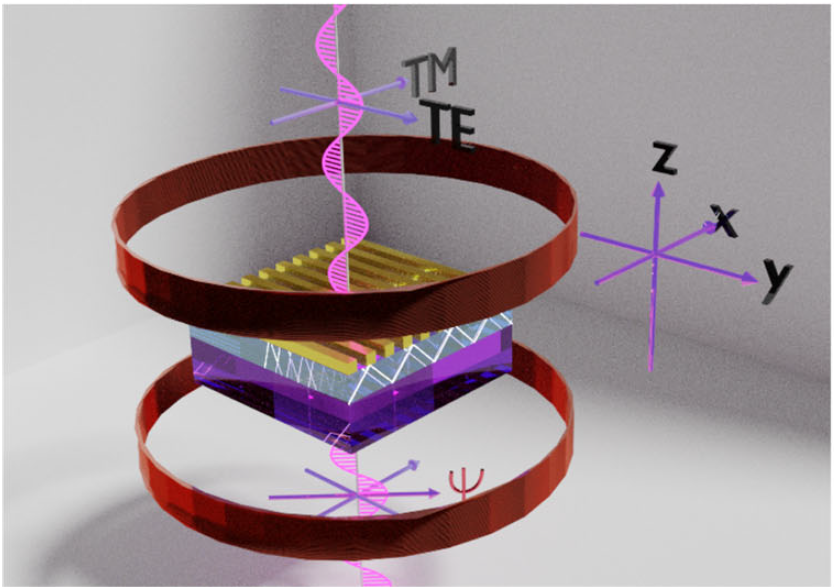
\includegraphics[width=\linewidth, height=140px]{Figures/figure1a.png}
		\end{subfigure}
		\caption{\textbf{The waveguide magneto-plasmonic crystal (WMPC).} \textbf{(a)} schematic illustration of the WMPC system. The direction of the transverse magnetic TM $(x)$ and transverse electric TE $(y)$ polarized light electric fields are perpendicular and parallel (respectively) to the axis of the Au gratings in the WMPC.}
		\label{fig:figure1}
	\end{figure}
	\FloatBarrier
	\par
	Here in th figure \ref{fig:figure3} indicates that the amplification of the weak Faraday effect arises due to the near destructive interference of the TE polarized quasiguided mode with the continuum mode at close vicinity of the Fano spectral dip and it takes place at the expense of the total intensity signal, which is a universal signature of WVA. The simulated Faraday rotation $\psi$ for the WMPCS having $d = 550 nm$ is also observed to follow the $(\propto \cot \alpha \epsilon_a  \sim \frac{\alpha}{\epsilon_a})$ ( $\alpha$ is a small rotation ) behavior (Fig. \ref{fig:figure3}) as predicted by the natural WVA formalism. A quantitative comparison of the amplified Faraday rotation $\psi$ with the exact theoretical predictions of natural WVA of Faraday effect in Fano resonance (in details\cite{1.paper}) shows good agreement. This confirms that natural WVA in Fano resonance is the underlying reason for the enhancement of weak Faraday effect in the WMPC system having a value of periodicity $d = 550 nm$.
	
	
	\begin{figure}[hbt!]
		\centering
		\begin{subfigure}[]{.49\linewidth}
			\centering
			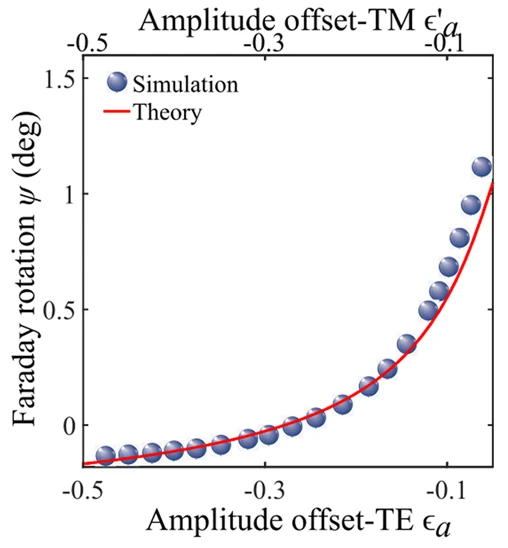
\includegraphics[width=\linewidth]{Figures/figure3a.png}
		\end{subfigure}
		\caption{\textbf{Natural weak value amplification result .} The variation of the Faraday rotation $\psi$ as a function of amplitude offset parameters $\epsilon_a$ of TE and $\epsilon^{'}_a$ of TM waveguide modes (gray metallic balls) and the corresponding theoretical predictions of natural WVA (red solid line). The $\epsilon_a$and $\epsilon^{'}_a$ parameters are shown in the lower and upper X-axes, respectively. }
		\label{fig:figure3}
	\end{figure}
	\subsection{Measurement of valley coherence}
	\noindent
	\par
	The metal dichalcogenide system comprises Tungsten diselenide (WSe2) on top of a Hexagonal Boron Nitride(h-BN). The WSe2 is material that has valley coherence. A sharp resonance from valley coherence interference with the broad light forms a sharp asymmetric Fano resonance.
	\begin{figure}
		\centering
		\begin{subfigure}[]{.49\linewidth}
			\centering
			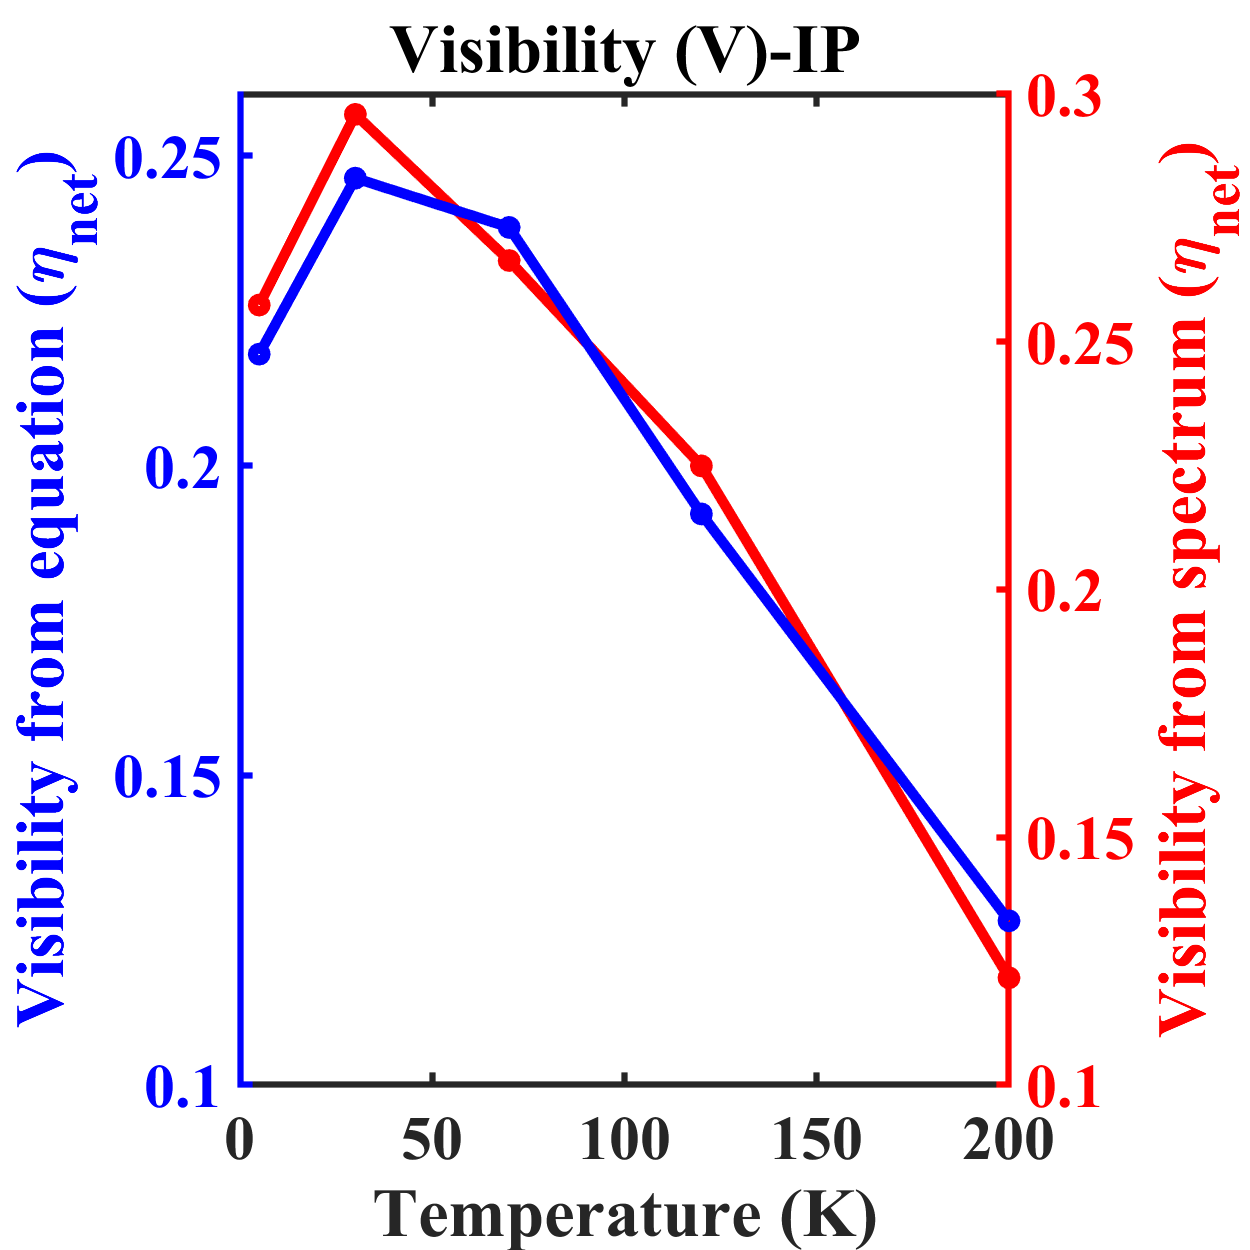
\includegraphics[width=\linewidth]{Figures/IP_V.png}
		\end{subfigure}
		\caption{\textbf{Valley coherence result .} The left y-axis (\textcolor{red}{red} color) is plotted the $\eta_{net} (\mathscr{V})$ calculated from the fitting equation (equation \ref{eqs:valley coherence Fano equation}). The right y-axis (\textcolor{blue}{blue} color) is plotted the $\eta_{net} (\mathscr{V})$ calculated from the peak and dip of the spectrum.}
		\label{fig:valley}
	\end{figure}
	\par 
	In the figure \ref{fig:valley}, we have calculated the visibility $(\mathscr{V})$ from the spectrum peak and dip position, we fit the equation \ref{eqs:valley coherence Fano equation} and calculated the visibility $(\mathscr{V})$ from the equation. In the figure, we have shown both visibility $(\mathscr{V})$ are comparable this is evidence of our theory. From the visibility $(\mathscr{V})$ we calculated the valley coherence. 
	
	\FloatBarrier
	\section{Summary}
	\noindent
	\par 
	In summary, our studies have unraveled different physical origins for the enhancement of Faraday rotation and ellipticity in magneto-plasmonic crystals. Natural WVA of weak Faraday effect that arises due to near destructive spectral domain interference in Fano resonance of the plasmonic crystals is identified as the primary mechanisms for enhancement with TE polarization excitation. These results are of both fundamental and applied interests. The quantitative understanding gained on the different physical mechanisms for the enhancement of the MO effects provides a useful recipe and a systematic approach for the optimization of the geometrical parameters of the WMPC towards achieving maximum enhancement of Faraday effects and for controlled tailoring of the MO responses of such hybrid systems. The different mechanisms for the enhancement of MO effects also indicate that the choice of input polarization state may provide an extra degree of freedom to optimally combine the two different mechanisms for the enhancement of MO response of such hybrid magneto-plasmonic systems. These may lead to optimized development of multifunctional nonreciprocal photonic nano-devices which potentially enhance their applications in optical isolation, modulation, rotation, magnetic field sensing, and so on. Moreover, the interferometric origin of natural WVA of Faraday effect also opens up the possibility of extending the philosophy to other interesting wave phenomena like electromagnetically induced transparency (EIT) and absorption (EIA), extraordinary optical transmission (EOT), which have common origin in fine interference effects. We are currently expanding our investigations in the aforementioned directions.
	
	\section{Future plan}
	\noindent
	\par 
	\subsection{Diffraction of a vector beam by a tilted aperture}
	\par 
	Spin-orbit interactions of the light beams are meaningful and exciting because of their fundamental nature and potential applications. We are investigating the spin-orbit interaction on the vector beam in a tilted aperture. Here, a tilted aperture breaks the system's symmetry, and due to this symmetry being broken, the spin-orbit interaction happens here.
	
	\subsection{Spin orbit interaction in turbid medium}
	\par 
	In turbid medium the conventional polarized light, scattered multiple number of times, is depolarized, and the depolarization rate depends strongly on the size and shape of scattering particles, as well as on the number of scattering events. In fact, the structure of light can be more complicated when the polarization of light across the laser beam can be radially or azimuthally polarized and carry orbital angular momentum. When  Laguerre-Gaussian (LG) beams, propagates in turbid  medium, either anisotropic or inhomogeneous, the spin or angular momentum are changed that leads to spin-orbit interaction. Such a spin-orbit interaction leads to the mutual influence of the polarization and the trajectory of the light propagation. We are investigating the spin-orbit interaction of  LG beams in a turbid medium.
	
	\printbibliography
\end{document}
